% ============================================================
% fig_proyeccion_embedding.tex — Proyección: one-hot → embedding
% Incluye tabla numérica + figura geométrica
% Uso: % ============================================================
% fig_proyeccion_embedding.tex — Proyección: one-hot → embedding
% Incluye tabla numérica + figura geométrica
% Uso: % ============================================================
% fig_proyeccion_embedding.tex — Proyección: one-hot → embedding
% Incluye tabla numérica + figura geométrica
% Uso: % ============================================================
% fig_proyeccion_embedding.tex — Proyección: one-hot → embedding
% Incluye tabla numérica + figura geométrica
% Uso: \input{figures/fig_proyeccion_embedding}
% ============================================================
\begin{figure}[H]
\centering

%──────────────────────────────────────────────────────────────
% PARTE SUPERIOR: tabla numérica de la proyección
%──────────────────────────────────────────────────────────────
\begin{tikzpicture}[
    cell/.style={draw=gray!40, minimum width=0.72cm, minimum height=0.60cm,
                 font=\scriptsize, inner sep=1pt},
    hdr/.style={font=\footnotesize\bfseries},
    hot/.style={fill=blue!50, text=white},
    emb/.style={fill=orange!20}
]

% ── Encabezado columnas ───────────────────────────────────
\node[hdr] at (-1.6, 2.8) {Token};
\node[hdr] at ( 1.4, 2.8) {One-hot $\bm{v}$ $\,(|\mathcal{V}|=4)$};
\node[hdr] at ( 5.6, 2.8) {Embedding $\bm{e} = E\bm{v}$ $\,(d_{\text{model}}=2)$};

% ── Fila: "gato" ─────────────────────────────────────────
\node[font=\small\itshape] at (-1.6, 2.1) {gato};
\foreach \v/\i in {1/0, 0/1, 0/2, 0/3}{
    \pgfmathparse{int(\v==1)}
    \ifnum\pgfmathresult=1
        \node[cell, hot] at (-0.3+\i*0.75, 2.1) {\v};
    \else
        \node[cell]      at (-0.3+\i*0.75, 2.1) {\v};
    \fi
}
\node[font=\Large] at (3.55, 2.1) {$\xrightarrow{\;E\;}$};
\node[cell, emb] at (4.6,  2.1) {0.8};
\node[cell, emb] at (5.35, 2.1) {0.3};

% ── Fila: "perro" ────────────────────────────────────────
\node[font=\small\itshape] at (-1.6, 1.3) {perro};
\foreach \v/\i in {0/0, 1/1, 0/2, 0/3}{
    \pgfmathparse{int(\v==1)}
    \ifnum\pgfmathresult=1
        \node[cell, hot] at (-0.3+\i*0.75, 1.3) {\v};
    \else
        \node[cell]      at (-0.3+\i*0.75, 1.3) {\v};
    \fi
}
\node[font=\Large] at (3.55, 1.3) {$\xrightarrow{\;E\;}$};
\node[cell, emb] at (4.6,  1.3) {0.7};
\node[cell, emb] at (5.35, 1.3) {0.4};

% ── Fila: "auto" ─────────────────────────────────────────
\node[font=\small\itshape] at (-1.6, 0.5) {auto};
\foreach \v/\i in {0/0, 0/1, 1/2, 0/3}{
    \pgfmathparse{int(\v==1)}
    \ifnum\pgfmathresult=1
        \node[cell, hot] at (-0.3+\i*0.75, 0.5) {\v};
    \else
        \node[cell]      at (-0.3+\i*0.75, 0.5) {\v};
    \fi
}
\node[font=\Large] at (3.55, 0.5) {$\xrightarrow{\;E\;}$};
\node[cell, emb] at (4.6,  0.5) {0.1};
\node[cell, emb] at (5.35, 0.5) {0.9};

% ── Fila: "tren" ─────────────────────────────────────────
\node[font=\small\itshape] at (-1.6, -0.3) {tren};
\foreach \v/\i in {0/0, 0/1, 0/2, 1/3}{
    \pgfmathparse{int(\v==1)}
    \ifnum\pgfmathresult=1
        \node[cell, hot] at (-0.3+\i*0.75, -0.3) {\v};
    \else
        \node[cell]      at (-0.3+\i*0.75, -0.3) {\v};
    \fi
}
\node[font=\Large] at (3.55, -0.3) {$\xrightarrow{\;E\;}$};
\node[cell, emb] at (4.6,  -0.3) {0.2};
\node[cell, emb] at (5.35, -0.3) {0.8};

% ── Nota ─────────────────────────────────────────────────
\node[font=\tiny, gray, align=left] at (1.8, -0.85)
    {La representación one-hot tiene distancia idéntica entre todos los pares.
     El embedding captura similitud.};

\end{tikzpicture}

\vspace{0.8em}

%──────────────────────────────────────────────────────────────
% PARTE INFERIOR: figura geométrica del espacio de embeddings
%──────────────────────────────────────────────────────────────
\begin{tikzpicture}[scale=1.05]

\node[font=\small\bfseries, gray] at (3.0, 4.1) {Espacio de embeddings ($d_{\text{model}}=2$)};

% Ejes
\draw[-{Stealth}] (-0.2, 0) -- (4.5, 0) node[right, font=\scriptsize] {dim 1};
\draw[-{Stealth}] (0, -0.2) -- (0, 4.0) node[above, font=\scriptsize] {dim 2};

% Puntos
\fill[red!60]    (3.2, 1.2) circle (4pt) node[right, font=\footnotesize] {\textit{gato}  $(0.8,\,0.3)$};
\fill[red!40]    (2.8, 1.6) circle (4pt) node[left,  font=\footnotesize] {\textit{perro} $(0.7,\,0.4)$};
\fill[blue!60]   (0.4, 3.6) circle (4pt) node[right, font=\footnotesize] {\textit{auto}  $(0.1,\,0.9)$};
\fill[blue!40]   (0.8, 3.2) circle (4pt) node[right, font=\footnotesize] {\textit{tren}  $(0.2,\,0.8)$};

% Elipses de agrupamiento
\draw[red!50,  dashed, thick] (3.0, 1.4) ellipse (0.55cm and 0.45cm);
\draw[blue!50, dashed, thick] (0.6, 3.4) ellipse (0.55cm and 0.45cm);

% Etiquetas de cluster
\node[font=\footnotesize, red!70]  at (3.75, 0.55) {animales};
\node[font=\footnotesize, blue!70] at (0.2,  2.55) {vehículos};

% Distancia entre clusters (flecha doble)
\draw[{Stealth}-{Stealth}, gray, thick] (2.55,1.45) -- (1.0,3.1);
\node[font=\tiny, gray, rotate=-52] at (1.65, 2.45) {distancia semántica};

% Nota
\node[font=\tiny, gray, align=center] at (3.0, -0.55)
    {Tokens semánticamente similares quedan próximos en el espacio.};

\end{tikzpicture}

\caption{Proyección de tokens mediante embeddings. \textbf{Arriba:} cada token
se representa primero como un vector \textit{one-hot} disperso y luego se
multiplica por la matriz de embeddings $E$, obteniendo un vector denso de
dimensión $d_{\text{model}}$. \textbf{Abajo:} en el espacio resultante, los
tokens semánticamente relacionados (\textit{gato}/\textit{perro},
\textit{auto}/\textit{tren}) quedan agrupados, mientras que categorías
distintas se separan geométricamente. Los valores numéricos son ilustrativos.}
\label{fig:proyeccion_embedding}
\end{figure}

% ============================================================
\begin{figure}[H]
\centering

%──────────────────────────────────────────────────────────────
% PARTE SUPERIOR: tabla numérica de la proyección
%──────────────────────────────────────────────────────────────
\begin{tikzpicture}[
    cell/.style={draw=gray!40, minimum width=0.72cm, minimum height=0.60cm,
                 font=\scriptsize, inner sep=1pt},
    hdr/.style={font=\footnotesize\bfseries},
    hot/.style={fill=blue!50, text=white},
    emb/.style={fill=orange!20}
]

% ── Encabezado columnas ───────────────────────────────────
\node[hdr] at (-1.6, 2.8) {Token};
\node[hdr] at ( 1.4, 2.8) {One-hot $\bm{v}$ $\,(|\mathcal{V}|=4)$};
\node[hdr] at ( 5.6, 2.8) {Embedding $\bm{e} = E\bm{v}$ $\,(d_{\text{model}}=2)$};

% ── Fila: "gato" ─────────────────────────────────────────
\node[font=\small\itshape] at (-1.6, 2.1) {gato};
\foreach \v/\i in {1/0, 0/1, 0/2, 0/3}{
    \pgfmathparse{int(\v==1)}
    \ifnum\pgfmathresult=1
        \node[cell, hot] at (-0.3+\i*0.75, 2.1) {\v};
    \else
        \node[cell]      at (-0.3+\i*0.75, 2.1) {\v};
    \fi
}
\node[font=\Large] at (3.55, 2.1) {$\xrightarrow{\;E\;}$};
\node[cell, emb] at (4.6,  2.1) {0.8};
\node[cell, emb] at (5.35, 2.1) {0.3};

% ── Fila: "perro" ────────────────────────────────────────
\node[font=\small\itshape] at (-1.6, 1.3) {perro};
\foreach \v/\i in {0/0, 1/1, 0/2, 0/3}{
    \pgfmathparse{int(\v==1)}
    \ifnum\pgfmathresult=1
        \node[cell, hot] at (-0.3+\i*0.75, 1.3) {\v};
    \else
        \node[cell]      at (-0.3+\i*0.75, 1.3) {\v};
    \fi
}
\node[font=\Large] at (3.55, 1.3) {$\xrightarrow{\;E\;}$};
\node[cell, emb] at (4.6,  1.3) {0.7};
\node[cell, emb] at (5.35, 1.3) {0.4};

% ── Fila: "auto" ─────────────────────────────────────────
\node[font=\small\itshape] at (-1.6, 0.5) {auto};
\foreach \v/\i in {0/0, 0/1, 1/2, 0/3}{
    \pgfmathparse{int(\v==1)}
    \ifnum\pgfmathresult=1
        \node[cell, hot] at (-0.3+\i*0.75, 0.5) {\v};
    \else
        \node[cell]      at (-0.3+\i*0.75, 0.5) {\v};
    \fi
}
\node[font=\Large] at (3.55, 0.5) {$\xrightarrow{\;E\;}$};
\node[cell, emb] at (4.6,  0.5) {0.1};
\node[cell, emb] at (5.35, 0.5) {0.9};

% ── Fila: "tren" ─────────────────────────────────────────
\node[font=\small\itshape] at (-1.6, -0.3) {tren};
\foreach \v/\i in {0/0, 0/1, 0/2, 1/3}{
    \pgfmathparse{int(\v==1)}
    \ifnum\pgfmathresult=1
        \node[cell, hot] at (-0.3+\i*0.75, -0.3) {\v};
    \else
        \node[cell]      at (-0.3+\i*0.75, -0.3) {\v};
    \fi
}
\node[font=\Large] at (3.55, -0.3) {$\xrightarrow{\;E\;}$};
\node[cell, emb] at (4.6,  -0.3) {0.2};
\node[cell, emb] at (5.35, -0.3) {0.8};

% ── Nota ─────────────────────────────────────────────────
\node[font=\tiny, gray, align=left] at (1.8, -0.85)
    {La representación one-hot tiene distancia idéntica entre todos los pares.
     El embedding captura similitud.};

\end{tikzpicture}

\vspace{0.8em}

%──────────────────────────────────────────────────────────────
% PARTE INFERIOR: figura geométrica del espacio de embeddings
%──────────────────────────────────────────────────────────────
\begin{tikzpicture}[scale=1.05]

\node[font=\small\bfseries, gray] at (3.0, 4.1) {Espacio de embeddings ($d_{\text{model}}=2$)};

% Ejes
\draw[-{Stealth}] (-0.2, 0) -- (4.5, 0) node[right, font=\scriptsize] {dim 1};
\draw[-{Stealth}] (0, -0.2) -- (0, 4.0) node[above, font=\scriptsize] {dim 2};

% Puntos
\fill[red!60]    (3.2, 1.2) circle (4pt) node[right, font=\footnotesize] {\textit{gato}  $(0.8,\,0.3)$};
\fill[red!40]    (2.8, 1.6) circle (4pt) node[left,  font=\footnotesize] {\textit{perro} $(0.7,\,0.4)$};
\fill[blue!60]   (0.4, 3.6) circle (4pt) node[right, font=\footnotesize] {\textit{auto}  $(0.1,\,0.9)$};
\fill[blue!40]   (0.8, 3.2) circle (4pt) node[right, font=\footnotesize] {\textit{tren}  $(0.2,\,0.8)$};

% Elipses de agrupamiento
\draw[red!50,  dashed, thick] (3.0, 1.4) ellipse (0.55cm and 0.45cm);
\draw[blue!50, dashed, thick] (0.6, 3.4) ellipse (0.55cm and 0.45cm);

% Etiquetas de cluster
\node[font=\footnotesize, red!70]  at (3.75, 0.55) {animales};
\node[font=\footnotesize, blue!70] at (0.2,  2.55) {vehículos};

% Distancia entre clusters (flecha doble)
\draw[{Stealth}-{Stealth}, gray, thick] (2.55,1.45) -- (1.0,3.1);
\node[font=\tiny, gray, rotate=-52] at (1.65, 2.45) {distancia semántica};

% Nota
\node[font=\tiny, gray, align=center] at (3.0, -0.55)
    {Tokens semánticamente similares quedan próximos en el espacio.};

\end{tikzpicture}

\caption{Proyección de tokens mediante embeddings. \textbf{Arriba:} cada token
se representa primero como un vector \textit{one-hot} disperso y luego se
multiplica por la matriz de embeddings $E$, obteniendo un vector denso de
dimensión $d_{\text{model}}$. \textbf{Abajo:} en el espacio resultante, los
tokens semánticamente relacionados (\textit{gato}/\textit{perro},
\textit{auto}/\textit{tren}) quedan agrupados, mientras que categorías
distintas se separan geométricamente. Los valores numéricos son ilustrativos.}
\label{fig:proyeccion_embedding}
\end{figure}

% ============================================================
\begin{figure}[H]
\centering

%──────────────────────────────────────────────────────────────
% PARTE SUPERIOR: tabla numérica de la proyección
%──────────────────────────────────────────────────────────────
\begin{tikzpicture}[
    cell/.style={draw=gray!40, minimum width=0.72cm, minimum height=0.60cm,
                 font=\scriptsize, inner sep=1pt},
    hdr/.style={font=\footnotesize\bfseries},
    hot/.style={fill=blue!50, text=white},
    emb/.style={fill=orange!20}
]

% ── Encabezado columnas ───────────────────────────────────
\node[hdr] at (-1.6, 2.8) {Token};
\node[hdr] at ( 1.4, 2.8) {One-hot $\bm{v}$ $\,(|\mathcal{V}|=4)$};
\node[hdr] at ( 5.6, 2.8) {Embedding $\bm{e} = E\bm{v}$ $\,(d_{\text{model}}=2)$};

% ── Fila: "gato" ─────────────────────────────────────────
\node[font=\small\itshape] at (-1.6, 2.1) {gato};
\foreach \v/\i in {1/0, 0/1, 0/2, 0/3}{
    \pgfmathparse{int(\v==1)}
    \ifnum\pgfmathresult=1
        \node[cell, hot] at (-0.3+\i*0.75, 2.1) {\v};
    \else
        \node[cell]      at (-0.3+\i*0.75, 2.1) {\v};
    \fi
}
\node[font=\Large] at (3.55, 2.1) {$\xrightarrow{\;E\;}$};
\node[cell, emb] at (4.6,  2.1) {0.8};
\node[cell, emb] at (5.35, 2.1) {0.3};

% ── Fila: "perro" ────────────────────────────────────────
\node[font=\small\itshape] at (-1.6, 1.3) {perro};
\foreach \v/\i in {0/0, 1/1, 0/2, 0/3}{
    \pgfmathparse{int(\v==1)}
    \ifnum\pgfmathresult=1
        \node[cell, hot] at (-0.3+\i*0.75, 1.3) {\v};
    \else
        \node[cell]      at (-0.3+\i*0.75, 1.3) {\v};
    \fi
}
\node[font=\Large] at (3.55, 1.3) {$\xrightarrow{\;E\;}$};
\node[cell, emb] at (4.6,  1.3) {0.7};
\node[cell, emb] at (5.35, 1.3) {0.4};

% ── Fila: "auto" ─────────────────────────────────────────
\node[font=\small\itshape] at (-1.6, 0.5) {auto};
\foreach \v/\i in {0/0, 0/1, 1/2, 0/3}{
    \pgfmathparse{int(\v==1)}
    \ifnum\pgfmathresult=1
        \node[cell, hot] at (-0.3+\i*0.75, 0.5) {\v};
    \else
        \node[cell]      at (-0.3+\i*0.75, 0.5) {\v};
    \fi
}
\node[font=\Large] at (3.55, 0.5) {$\xrightarrow{\;E\;}$};
\node[cell, emb] at (4.6,  0.5) {0.1};
\node[cell, emb] at (5.35, 0.5) {0.9};

% ── Fila: "tren" ─────────────────────────────────────────
\node[font=\small\itshape] at (-1.6, -0.3) {tren};
\foreach \v/\i in {0/0, 0/1, 0/2, 1/3}{
    \pgfmathparse{int(\v==1)}
    \ifnum\pgfmathresult=1
        \node[cell, hot] at (-0.3+\i*0.75, -0.3) {\v};
    \else
        \node[cell]      at (-0.3+\i*0.75, -0.3) {\v};
    \fi
}
\node[font=\Large] at (3.55, -0.3) {$\xrightarrow{\;E\;}$};
\node[cell, emb] at (4.6,  -0.3) {0.2};
\node[cell, emb] at (5.35, -0.3) {0.8};

% ── Nota ─────────────────────────────────────────────────
\node[font=\tiny, gray, align=left] at (1.8, -0.85)
    {La representación one-hot tiene distancia idéntica entre todos los pares.
     El embedding captura similitud.};

\end{tikzpicture}

\vspace{0.8em}

%──────────────────────────────────────────────────────────────
% PARTE INFERIOR: figura geométrica del espacio de embeddings
%──────────────────────────────────────────────────────────────
\begin{tikzpicture}[scale=1.05]

\node[font=\small\bfseries, gray] at (3.0, 4.1) {Espacio de embeddings ($d_{\text{model}}=2$)};

% Ejes
\draw[-{Stealth}] (-0.2, 0) -- (4.5, 0) node[right, font=\scriptsize] {dim 1};
\draw[-{Stealth}] (0, -0.2) -- (0, 4.0) node[above, font=\scriptsize] {dim 2};

% Puntos
\fill[red!60]    (3.2, 1.2) circle (4pt) node[right, font=\footnotesize] {\textit{gato}  $(0.8,\,0.3)$};
\fill[red!40]    (2.8, 1.6) circle (4pt) node[left,  font=\footnotesize] {\textit{perro} $(0.7,\,0.4)$};
\fill[blue!60]   (0.4, 3.6) circle (4pt) node[right, font=\footnotesize] {\textit{auto}  $(0.1,\,0.9)$};
\fill[blue!40]   (0.8, 3.2) circle (4pt) node[right, font=\footnotesize] {\textit{tren}  $(0.2,\,0.8)$};

% Elipses de agrupamiento
\draw[red!50,  dashed, thick] (3.0, 1.4) ellipse (0.55cm and 0.45cm);
\draw[blue!50, dashed, thick] (0.6, 3.4) ellipse (0.55cm and 0.45cm);

% Etiquetas de cluster
\node[font=\footnotesize, red!70]  at (3.75, 0.55) {animales};
\node[font=\footnotesize, blue!70] at (0.2,  2.55) {vehículos};

% Distancia entre clusters (flecha doble)
\draw[{Stealth}-{Stealth}, gray, thick] (2.55,1.45) -- (1.0,3.1);
\node[font=\tiny, gray, rotate=-52] at (1.65, 2.45) {distancia semántica};

% Nota
\node[font=\tiny, gray, align=center] at (3.0, -0.55)
    {Tokens semánticamente similares quedan próximos en el espacio.};

\end{tikzpicture}

\caption{Proyección de tokens mediante embeddings. \textbf{Arriba:} cada token
se representa primero como un vector \textit{one-hot} disperso y luego se
multiplica por la matriz de embeddings $E$, obteniendo un vector denso de
dimensión $d_{\text{model}}$. \textbf{Abajo:} en el espacio resultante, los
tokens semánticamente relacionados (\textit{gato}/\textit{perro},
\textit{auto}/\textit{tren}) quedan agrupados, mientras que categorías
distintas se separan geométricamente. Los valores numéricos son ilustrativos.}
\label{fig:proyeccion_embedding}
\end{figure}

% ============================================================
\begin{figure}[H]
\centering

%──────────────────────────────────────────────────────────────
% PARTE SUPERIOR: tabla numérica de la proyección
%──────────────────────────────────────────────────────────────
\begin{tikzpicture}[
    cell/.style={draw=gray!40, minimum width=0.72cm, minimum height=0.60cm,
                 font=\scriptsize, inner sep=1pt},
    hdr/.style={font=\footnotesize\bfseries},
    hot/.style={fill=blue!50, text=white},
    emb/.style={fill=orange!20}
]

% ── Encabezado columnas ───────────────────────────────────
\node[hdr] at (-1.6, 2.8) {Token};
\node[hdr] at ( 1.4, 2.8) {One-hot $\bm{v}$ $\,(|\mathcal{V}|=4)$};
\node[hdr] at ( 5.6, 2.8) {Embedding $\bm{e} = E\bm{v}$ $\,(d_{\text{model}}=2)$};

% ── Fila: "gato" ─────────────────────────────────────────
\node[font=\small\itshape] at (-1.6, 2.1) {gato};
\foreach \v/\i in {1/0, 0/1, 0/2, 0/3}{
    \pgfmathparse{int(\v==1)}
    \ifnum\pgfmathresult=1
        \node[cell, hot] at (-0.3+\i*0.75, 2.1) {\v};
    \else
        \node[cell]      at (-0.3+\i*0.75, 2.1) {\v};
    \fi
}
\node[font=\Large] at (3.55, 2.1) {$\xrightarrow{\;E\;}$};
\node[cell, emb] at (4.6,  2.1) {0.8};
\node[cell, emb] at (5.35, 2.1) {0.3};

% ── Fila: "perro" ────────────────────────────────────────
\node[font=\small\itshape] at (-1.6, 1.3) {perro};
\foreach \v/\i in {0/0, 1/1, 0/2, 0/3}{
    \pgfmathparse{int(\v==1)}
    \ifnum\pgfmathresult=1
        \node[cell, hot] at (-0.3+\i*0.75, 1.3) {\v};
    \else
        \node[cell]      at (-0.3+\i*0.75, 1.3) {\v};
    \fi
}
\node[font=\Large] at (3.55, 1.3) {$\xrightarrow{\;E\;}$};
\node[cell, emb] at (4.6,  1.3) {0.7};
\node[cell, emb] at (5.35, 1.3) {0.4};

% ── Fila: "auto" ─────────────────────────────────────────
\node[font=\small\itshape] at (-1.6, 0.5) {auto};
\foreach \v/\i in {0/0, 0/1, 1/2, 0/3}{
    \pgfmathparse{int(\v==1)}
    \ifnum\pgfmathresult=1
        \node[cell, hot] at (-0.3+\i*0.75, 0.5) {\v};
    \else
        \node[cell]      at (-0.3+\i*0.75, 0.5) {\v};
    \fi
}
\node[font=\Large] at (3.55, 0.5) {$\xrightarrow{\;E\;}$};
\node[cell, emb] at (4.6,  0.5) {0.1};
\node[cell, emb] at (5.35, 0.5) {0.9};

% ── Fila: "tren" ─────────────────────────────────────────
\node[font=\small\itshape] at (-1.6, -0.3) {tren};
\foreach \v/\i in {0/0, 0/1, 0/2, 1/3}{
    \pgfmathparse{int(\v==1)}
    \ifnum\pgfmathresult=1
        \node[cell, hot] at (-0.3+\i*0.75, -0.3) {\v};
    \else
        \node[cell]      at (-0.3+\i*0.75, -0.3) {\v};
    \fi
}
\node[font=\Large] at (3.55, -0.3) {$\xrightarrow{\;E\;}$};
\node[cell, emb] at (4.6,  -0.3) {0.2};
\node[cell, emb] at (5.35, -0.3) {0.8};

% ── Nota ─────────────────────────────────────────────────
\node[font=\tiny, gray, align=left] at (1.8, -0.85)
    {La representación one-hot tiene distancia idéntica entre todos los pares.
     El embedding captura similitud.};

\end{tikzpicture}

\vspace{0.8em}

%──────────────────────────────────────────────────────────────
% PARTE INFERIOR: figura geométrica del espacio de embeddings
%──────────────────────────────────────────────────────────────
\begin{tikzpicture}[scale=1.05]

\node[font=\small\bfseries, gray] at (3.0, 4.1) {Espacio de embeddings ($d_{\text{model}}=2$)};

% Ejes
\draw[-{Stealth}] (-0.2, 0) -- (4.5, 0) node[right, font=\scriptsize] {dim 1};
\draw[-{Stealth}] (0, -0.2) -- (0, 4.0) node[above, font=\scriptsize] {dim 2};

% Puntos
\fill[red!60]    (3.2, 1.2) circle (4pt) node[right, font=\footnotesize] {\textit{gato}  $(0.8,\,0.3)$};
\fill[red!40]    (2.8, 1.6) circle (4pt) node[left,  font=\footnotesize] {\textit{perro} $(0.7,\,0.4)$};
\fill[blue!60]   (0.4, 3.6) circle (4pt) node[right, font=\footnotesize] {\textit{auto}  $(0.1,\,0.9)$};
\fill[blue!40]   (0.8, 3.2) circle (4pt) node[right, font=\footnotesize] {\textit{tren}  $(0.2,\,0.8)$};

% Elipses de agrupamiento
\draw[red!50,  dashed, thick] (3.0, 1.4) ellipse (0.55cm and 0.45cm);
\draw[blue!50, dashed, thick] (0.6, 3.4) ellipse (0.55cm and 0.45cm);

% Etiquetas de cluster
\node[font=\footnotesize, red!70]  at (3.75, 0.55) {animales};
\node[font=\footnotesize, blue!70] at (0.2,  2.55) {vehículos};

% Distancia entre clusters (flecha doble)
\draw[{Stealth}-{Stealth}, gray, thick] (2.55,1.45) -- (1.0,3.1);
\node[font=\tiny, gray, rotate=-52] at (1.65, 2.45) {distancia semántica};

% Nota
\node[font=\tiny, gray, align=center] at (3.0, -0.55)
    {Tokens semánticamente similares quedan próximos en el espacio.};

\end{tikzpicture}

\caption{Proyección de tokens mediante embeddings. \textbf{Arriba:} cada token
se representa primero como un vector \textit{one-hot} disperso y luego se
multiplica por la matriz de embeddings $E$, obteniendo un vector denso de
dimensión $d_{\text{model}}$. \textbf{Abajo:} en el espacio resultante, los
tokens semánticamente relacionados (\textit{gato}/\textit{perro},
\textit{auto}/\textit{tren}) quedan agrupados, mientras que categorías
distintas se separan geométricamente. Los valores numéricos son ilustrativos.}
\label{fig:proyeccion_embedding}
\end{figure}
